\begin{task}{381}
Пусть ребра графа \(G\) правильно раскрашены в цвета \(\{0,1,2,\ldots,k\}\). Предположим, в \(G\) есть ровно одно ребро цвета \(0\), его концы~--- \(u,v\). Пусть также известно, что для покраски ребер, инцидентных \(u\), использованы все цвета, кроме \(k\), а для покраски ребер, инцидентных \(v\),~--- все, кроме \(1\) и \(2\). Пусть \(\{u,w\}\)~--- ребро цвета \(1\). Оказалось, что для раскраски ребер, инцидентных \(w\), не использованы цвета \(0\) и \(2\). Докажите, что ребра \(G\) можно правильно раскрасить в \(k\) цветов.  
\end{task}

Разложим условие <<по полочкам>>:
\begin{enumerate}
    \item Граф \(G\) правильно раскрашен в \((k + 1)\) цвет. А мы хотим получить правильную раскраску в \(k\) цветов. По условию существует только одно ребро цвета \(0\)~--- это ребро \((u, v)\). \textbf{Если получится убрать ребро с цветом \(0\), тогда мы добьемся цели}.
    
    \item В условии очень подробно расписаны цвета ребер, инцидентных вершинам \(u, v, w\). Представим это в виде небольшой схемы для удобства восприятия:
    \begin{figure}[H]
        \centering
        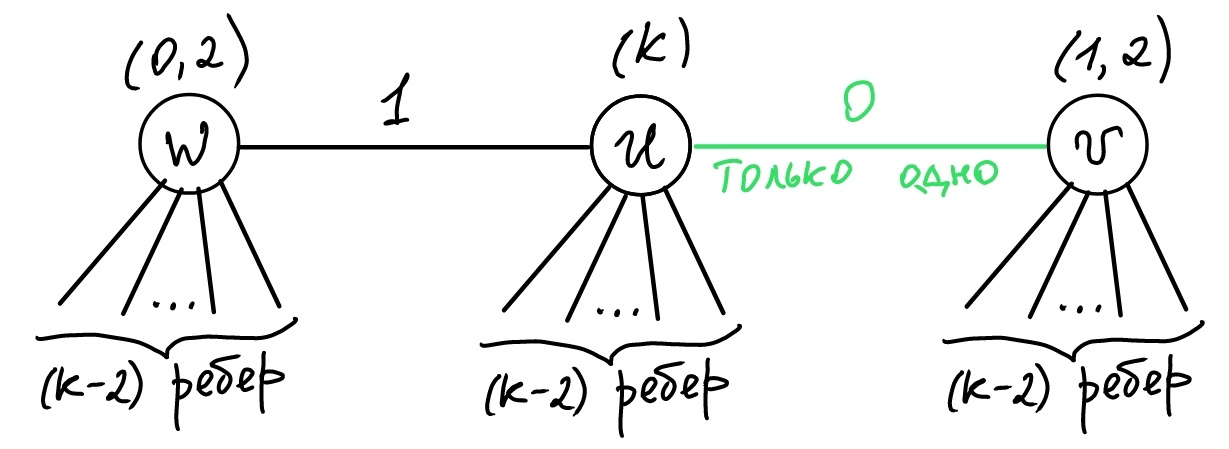
\includegraphics[scale=0.3]{Fall/img/solution-381_scheme.jpg}
        \caption{Условие в виде схемы.} \label{scheme 381}
    \end{figure}
    
    Далее будем пользоваться следующими обозначениями, часть которых изображена на схеме~\ref{scheme 381}:
    \begin{enumerate}
        \item Возле вершины в скобках будем показывать цвета, которые не встречаются среди цветов инцидентных ребер. Так по условию <<для покраски ребер, инцидентных \(u\), использованы все цвета, кроме \(k\)>>, значит, в скобках укажем только \(k\). Аналогично из условия возле вершины \(v\) указаны цвета \(1, 2\), возле вершины \(w\)~--- цвета \(0, 2\);
        
        \item Ребро, помеченное цветом \(0\) единственно. Далее будем обозначать его \emph{нуль-ребро}.
    \end{enumerate}
\end{enumerate}

Чтобы убрать \emph{нуль-ребро}, нужно в конечном счете пометить его каким-либо другим цветом. Сразу сделать это не получится, иначе нарушится условие правильной раскраски. Тогда введем операцию обмена цветами (\emph{swap}) у двух ребер, инцидентных одной вершине. И наложим важное ограничение, чтобы раскраска после обмена оставалась правильной:
\begin{figure}[H]
    \centering
    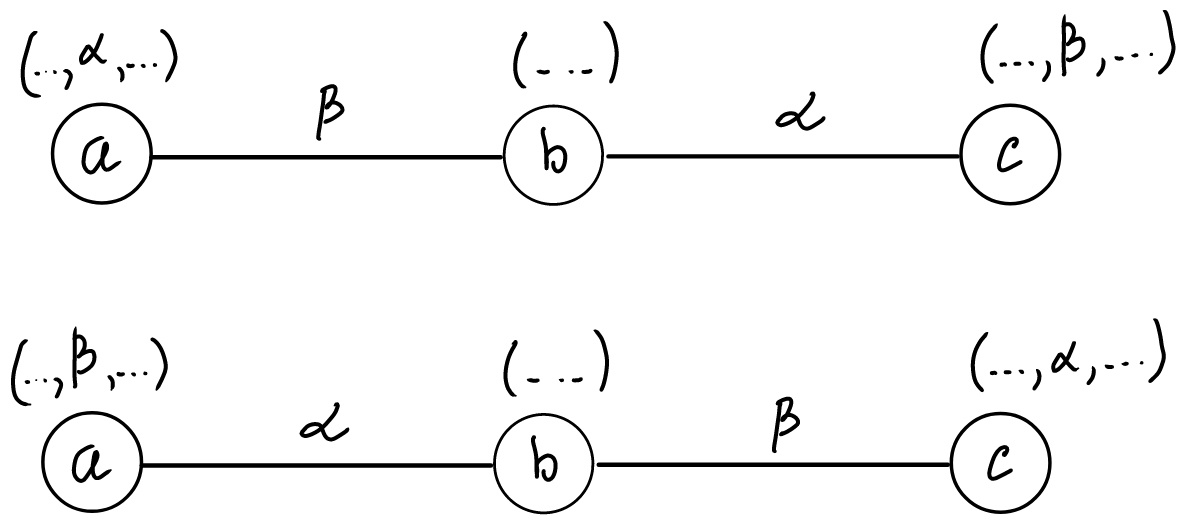
\includegraphics[scale=0.2]{Fall/img/solution-381_swap.jpg}
\end{figure}

Обмен цветами ребер \((a, b) \Leftrightarrow \beta\) и \((b, c) \Leftrightarrow \alpha\) сохранит условие правильной раскраски, если вершина \(a\) не имеет цвета \(\alpha\), а вершина \(c\) не имеет цвета \(\beta\).

\emph{Заметка:} мы будем использовать \emph{swap} только с \emph{нуль-ребром}, за цветом которого следить не нужно, потому что вершины, не инцидентные \emph{нуль-ребру}, гарантированно не будут иметь цвета \(0\).

Когда мы сможем заменить цвет \emph{нуль-ребра}? Когда возникнет ситуация, при которой обе вершины, соединенные \emph{нуль-ребром}, не будут иметь один и тот же цвет, допустим, цвет \(m\). Тогда заменяем цвет \(0\) на цвет \(m\) и побеждаем. Назовем эту ситуацию \textbf{Победа}.

Теперь другой вопрос: как добиться такой ситуации? Попробуем вовлечь в игру с обменами цвета, которые упомянуты в условии~--- это \(\{0, 1, 2, k\}\). А ребра с остальными цветами просто <<выкинем>>, потому что они ни на что не будут влиять.

Итак, мы получили граф с четырьмя цветами и хотим сделать так, чтобы осталось только три цвета. Стартуем с \emph{нуль-ребра} и начинаем двигаться по цепи вида \((0-k-2-k-\ldots-)\) в сторону вершины \(v\) и далее:
\begin{figure}[H]
    \centering
    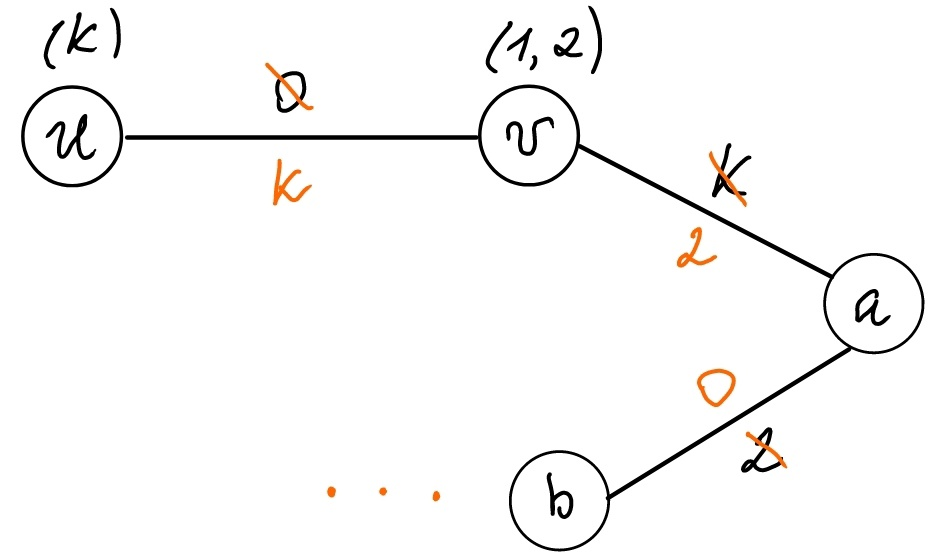
\includegraphics[scale=0.2]{Fall/img/solution-381_chain_begin.jpg}
\end{figure}

Если вдруг в процессе <<продвижения>> \emph{нуль-ребра} у вершины не окажется ребра цвета \(2\) после обмена \emph{ нуль-ребра} с ребром цвета \(k\), или наоборот~--- тогда алгоритм можно завершать, потому что мы пришли к ситуации \textbf{Победа}:
\begin{figure}[H]
    \centering
    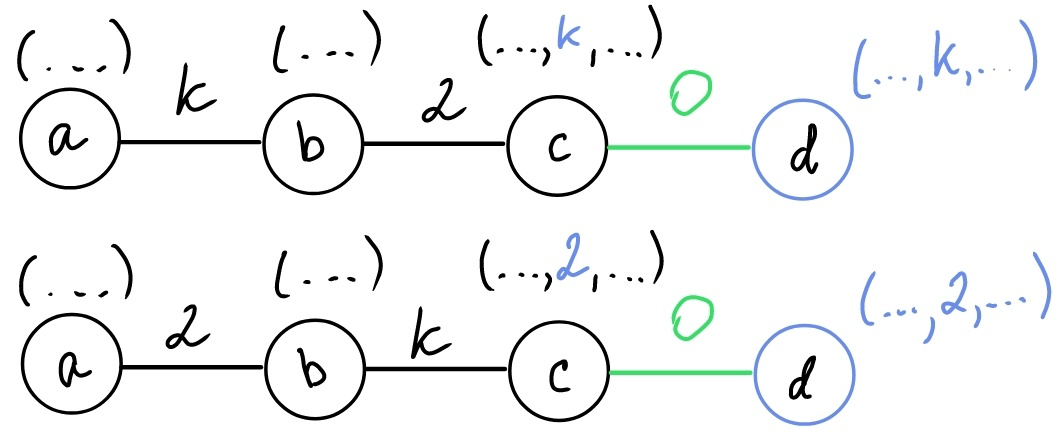
\includegraphics[scale=0.3]{Fall/img/solution-381_chain_end.jpg}
    \caption{Конец цепи, победа.} \label{chain win 381}
\end{figure}

Почему мы так смело утверждаем, что у вершины \(c\) нет цвета \(k\) или \(2\), необходимого для ситуации \textbf{Победа}~\eqref{chain win 381}? Дело в том, что при продвижении \emph{нуль-ребра} произошел <<сдвиг>> ребер с цветами \(2, k\), что привело к исчезновению одного из цветов у вершины \(c\). В первом случае от нее <<ушло>> ребро цвета \(k\:((b, c) \rightarrow (a, b))\); во втором~--- ребро цвета \(2\).

Но что если такой ситуации не случится? Бесконечной цепь быть не может, значит, она замкнется в стартовой вершине \(u\) и получится цикл:
\begin{figure}[H]
    \centering
    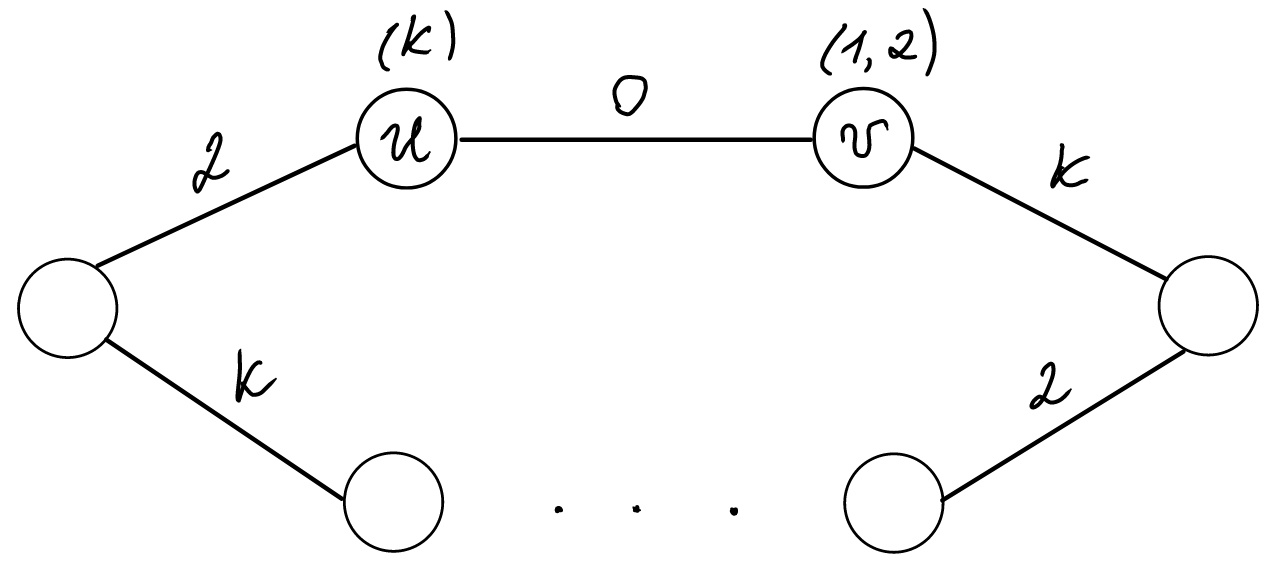
\includegraphics[scale=0.3]{Fall/img/solution-381_cycle.jpg}
    \caption{Цикл, включающий \emph{нуль-ребро} \((u, v)\)} \label{cycle 381}
\end{figure}

Это совсем не то, что нам нужно, ведь в цикле мы через какое угодно количество операций \emph{swap} не придем к ситуации \textbf{Победа}~\eqref{chain win 381}. Но и здесь мы можем извлечь выгоду. Допустим, что у нас не один такой цикл, а два: оба проходят через вершину \(u\); первый также проходит через вершину \(v\), второй, соответственно, через вершину \(w\); оба имеют общую часть \((u-t)\):
\begin{figure}[H]
    \centering
    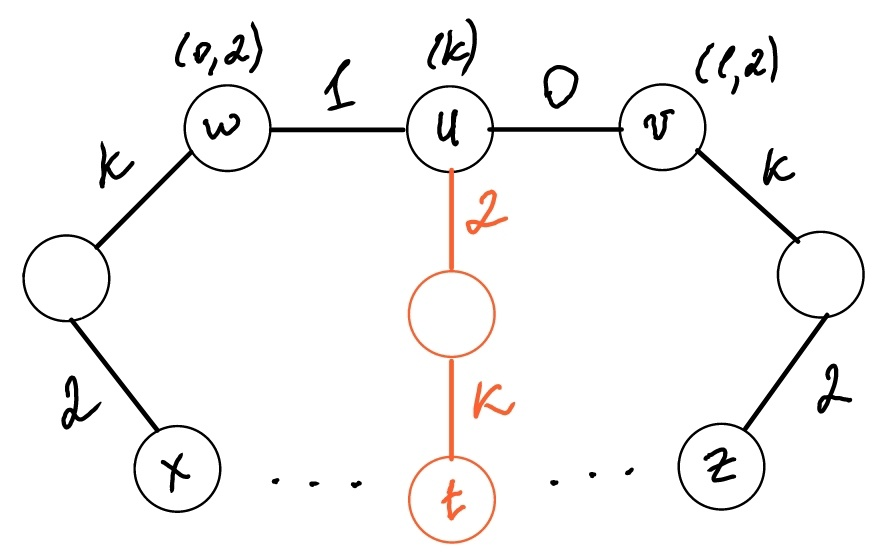
\includegraphics[scale=0.3]{Fall/img/solution-381_two_cycles.jpg}
    \caption{Два цикла быть не может.} \label{two cycles 381}
\end{figure}

Такая ситуация возможна? Нет! Ведь тогда каждый из циклов соединен с вершиной \(t\) ребром одного и того же цвета, другими словами, из вершины \(t\) исходят два ребра одного и того же цвета, а это противоречит правильности раскраски.

Используем это умозаключение. Допустим, образовался цикл~\ref{cycle 381}. Тогда если мы начнем обход из вершины \(u\), но уже через вершину \(w\), цепь замкнуть не сможем.

Но есть загвоздка: цепь \((u-w-\ldots-)\) не содержит \emph{нуль-ребра}. Эта проблема решается очень легко: сделаем \emph{swap} ребер \((u, v), (u, w)\). Это возможно, потому что \(u\) не содержит цвета \(1\), а \(w\) не содержит цвета \(0\). Более наглядно:
\begin{figure}[H]
    \centering
    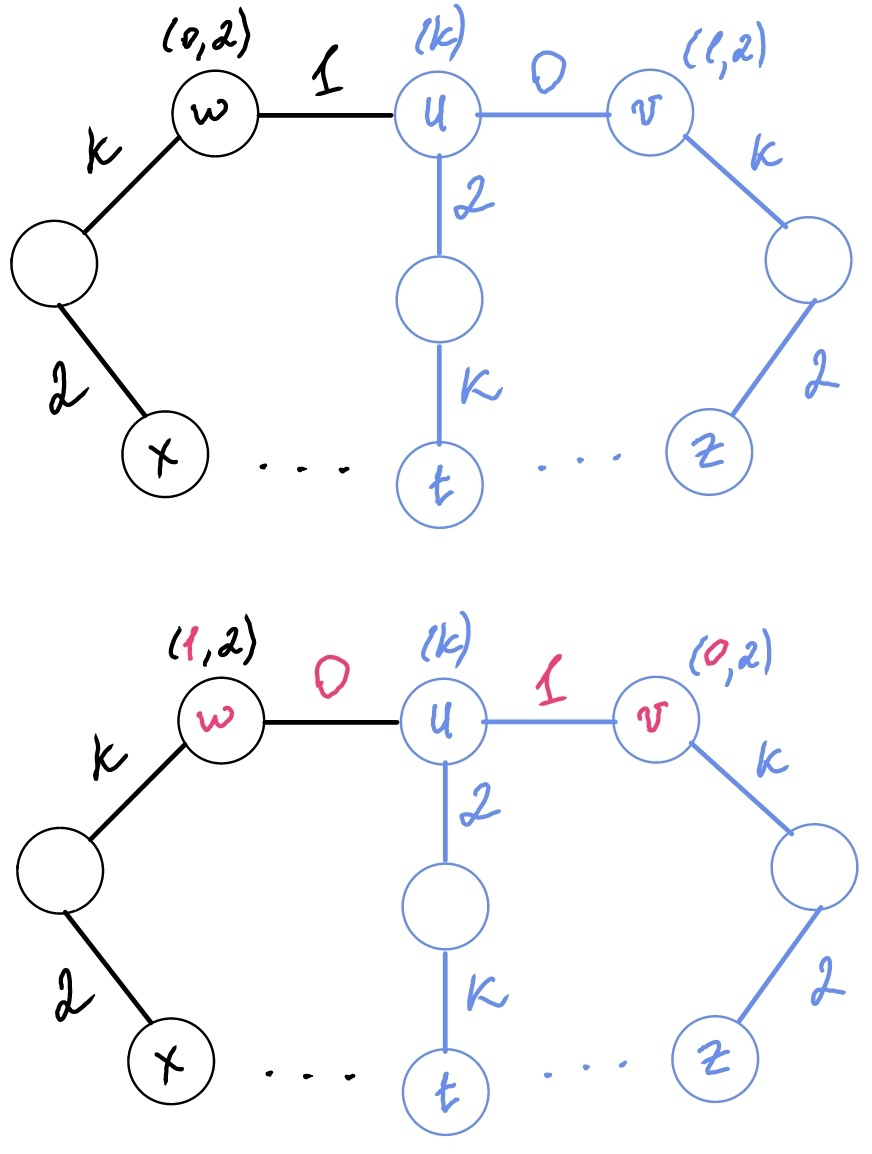
\includegraphics[scale=0.3]{Fall/img/solution-381_main_swap.jpg}
    \caption{Обмен ребер \((u, v), (u, w)\).} \label{main swap 381}
\end{figure}

Получаем цепь \((u-w-\ldots-)\), содержащую \emph{нуль-ребро}, которая никогда не замкнется, значит, обязательно придем к ситуации \textbf{Победа}~\eqref{chain win 381}~--- в противном случае цепь будет бесконечной.

\textbf{Коротко пробежимся по готовому плану:}

Нужно убрать \emph{нуль-ребро}. Для этого мы рассмотрели только ребра с цветами \(\{0, 1, 2, k\}\), потому что остальные не влияют на правильность раскраски по ходу алгоритма, ввели операцию \emph{swap} и приняли стратегию нахождения конечной цепи. Наша цель~--- ситуация \textbf{Победа}~\eqref{chain win 381}, при которой возможно изменение цвета \(0\) на любой другой с сохранением правильности раскраски. Дальше получаем несколько случаев:
\begin{enumerate}
    \item Цепь \((u-v-\ldots-)\) конечна. После серии операций \emph{swap} приходим к ситуации \textbf{Победа}~\eqref{chain win 381};
    
    \item Цепь \((u-v-\ldots-)\) замыкается~--- получаем цикл. Тогда:
    \begin{enumerate}
        \item Делаем \emph{swap} ребер \((u, v), (u, w)\) с сохранением правильности раскраски~\eqref{main swap 381};
        
        \item Рассматриваем всегда конечную цепь \((u-w-\ldots-)\), содержащую \emph{нуль-ребро}. После серии операций \emph{swap} приходим к ситуации \textbf{Победа}~\eqref{chain win 381}.
    \end{enumerate}
\end{enumerate}

После выполнения плана мы сохраняем правильность раскраски и перекрашиваем единственное ребро цвета \(0\) в один из цветов \(\{2, k\}\). Получаем искомую правильную раскраску графа \(G\) в \(k\) цветов.
